\documentclass[onecolumn]{preport}
\usepackage[dvipdfmx]{graphicx}
\graphicspath{{figs/}}

\title{知能情報論 レポート課題}
\author{48186619 伊藤秀朗}

\begin{document}

\pagestyle{empty}
\maketitle
\thispagestyle{empty}
\sloppy

\Large

\section{実現する知能機械の概要と応用先}
近年,コンピュータビジョンの技術はニューラルネットワークの発展により目覚ましい向上を遂げている.それらは柔軟性とロバスト性を兼ね備え,現実世界への適用においても有効性を示している.一方,ロボット分野での研究も年々進んでおり,例えばトヨタ自動車は生活支援ロボットの実用化に向けて,障害者や高齢者などの家庭内での自律生活をアシストするヒューマンサポートロボットHSR~\cite{hsr}(\figref{hsr})の開発を推進している.コンピュータビジョン技術のロボット分野への応用もなされるべき課題である.このレポートでは,HSRをはじめとするロボット間の認識を課題に挙げ,Mask R-CNN~\cite{mask-rcnn}を用いた学習手法でHSR自体の認識を行った.これにより,2台HSRやHSRと他のロボットによる複数ロボット協調の先駆けとなる.
\begin{figure}[htbp]
 \begin{center}
   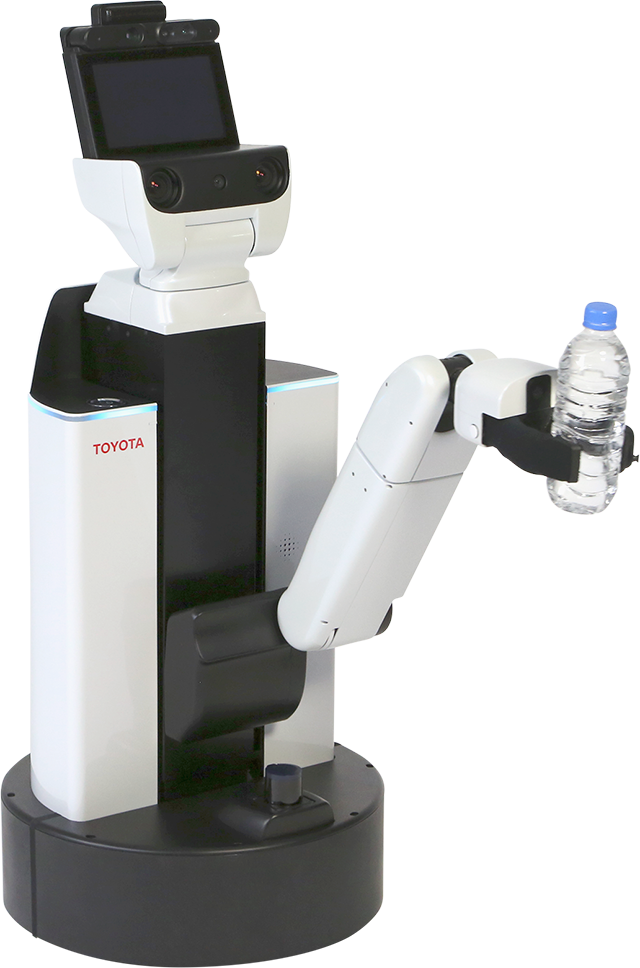
\includegraphics[width=0.20\columnwidth]{hsr.png}
   \caption{ヒューマンサポートロボットHSR~\cite{hsr}}
  \label{figure:hsr}
 \end{center}
\end{figure}

\section{学習手法と工夫点}
学習においてはchainerで記述されたMask R-CNNのネットワーク構造~\cite{mask-rcnn-wkentaro-github}を参考
・利用した.データセットには,自前で撮影および~\cite{labelme-wkentaro-github}を用いてアノテーションを行った30枚の画像とそのラベルデータを用いた.学習時のテストデータもこのデータセットと同じものを用いた.用意した画像とそのアノテーション画像の例を\figref{annotated}に示す.
\begin{figure}[htbp]
 \begin{center}
   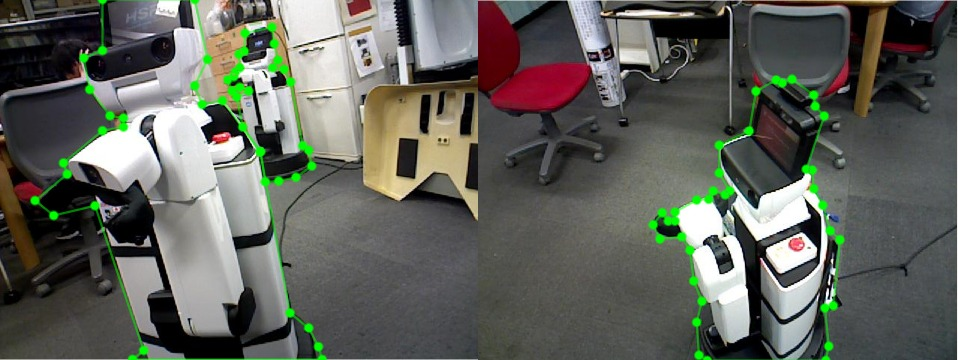
\includegraphics[width=0.6\columnwidth]{annotated.jpg}
   \caption{学習に用いたアノテーション画像}
  \label{figure:annotated}
 \end{center}
\end{figure}

\section{結果}
学習の結果を以下に示す.
\begin{figure}[htbp]
  \begin{center}
    \begin{minipage}{0.45\columnwidth}
      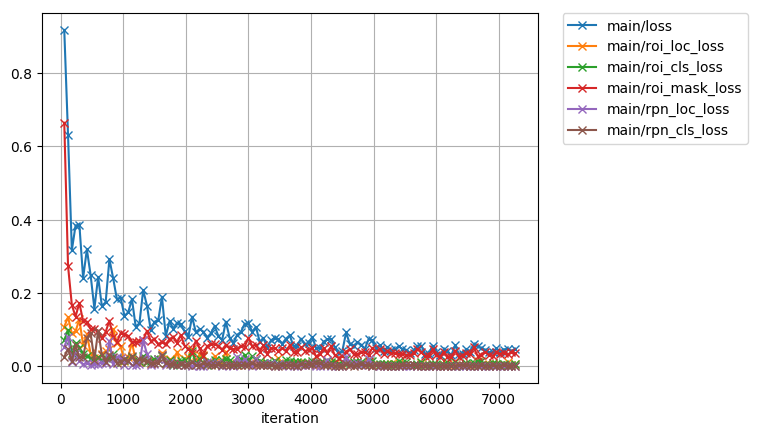
\includegraphics[width=\columnwidth]{loss.png}
      \caption{}
      \label{figure:loss}
    \end{minipage}
    %% \hspace{0.15\columnwidth}
    \begin{minipage}{0.45\columnwidth}
      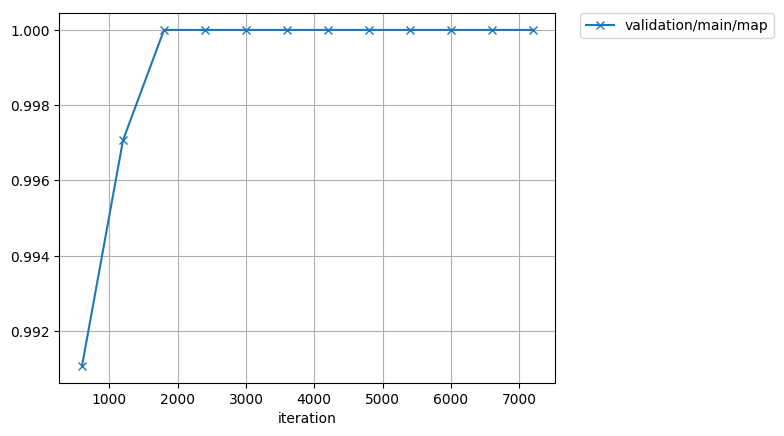
\includegraphics[width=\columnwidth]{accuracy.png}
      \caption{}
      \label{figure:accuracy}
    \end{minipage}
  \end{center}
\end{figure}

\begin{figure}[htbp]
 \begin{center}
   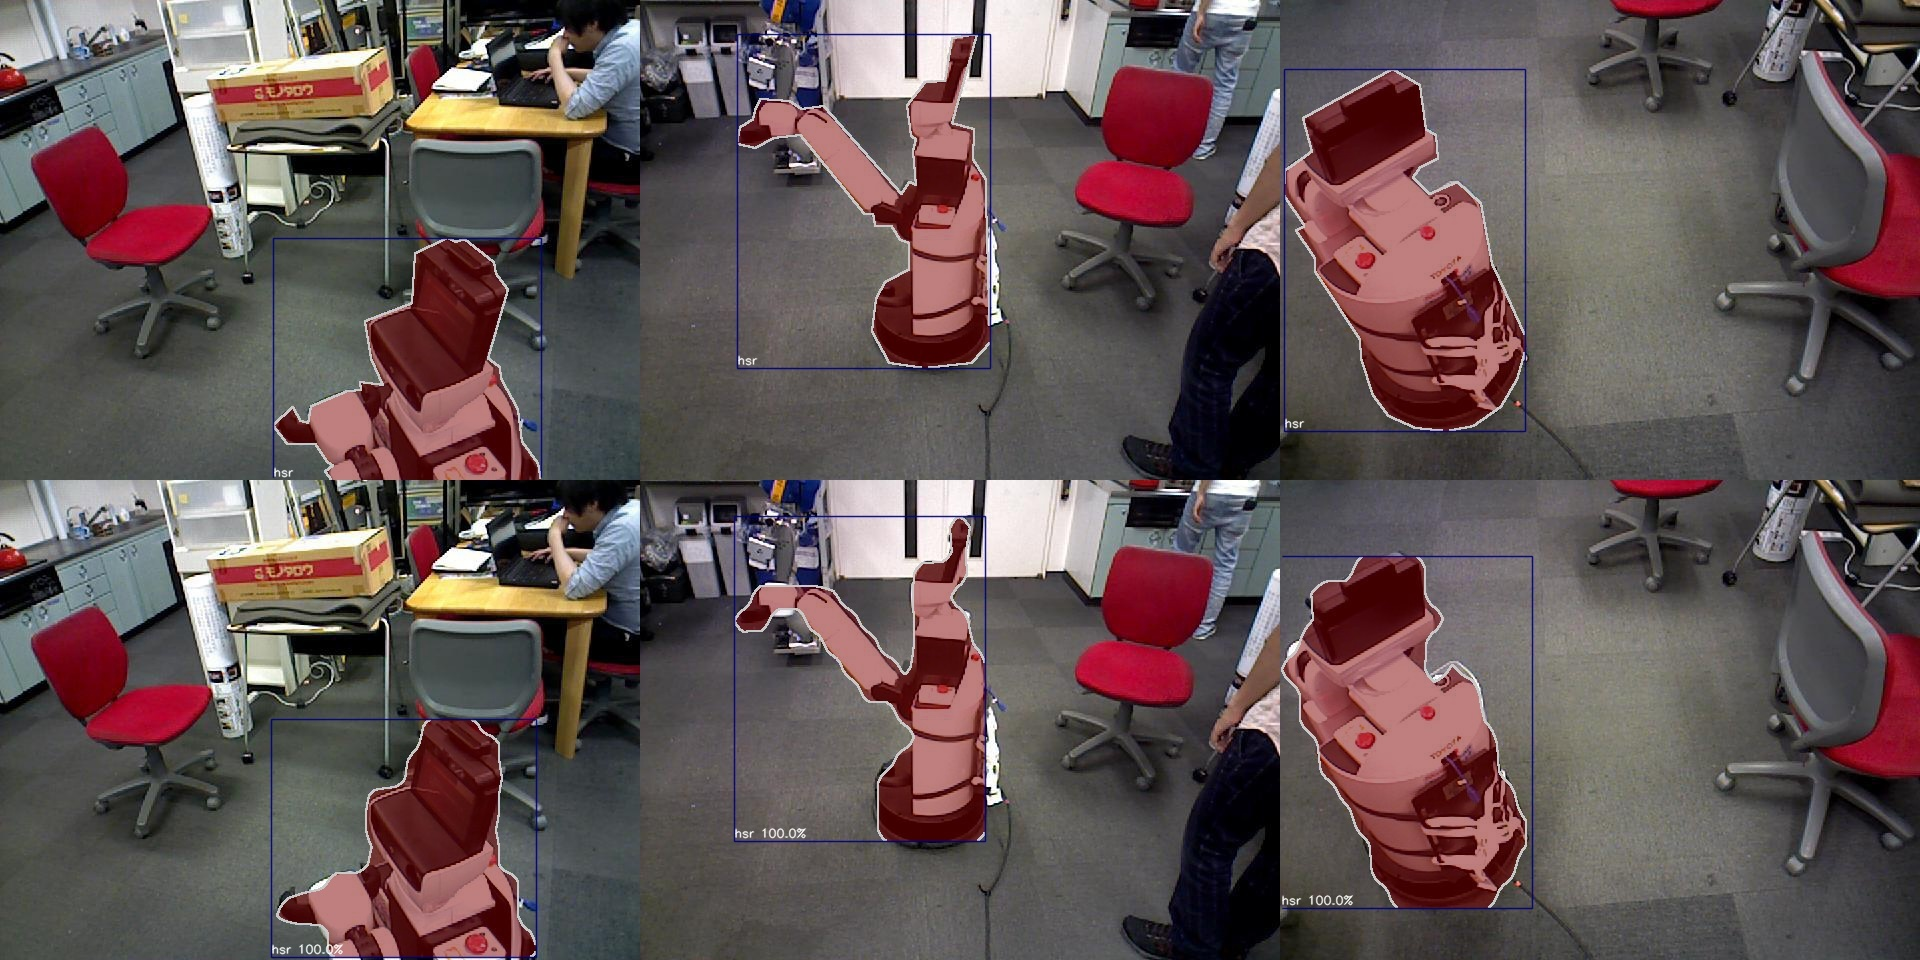
\includegraphics[width=0.5\columnwidth]{latest1.jpg}
   \caption{学習結果を可視化したもの.上が入力したアノテーション画像,下が学習されたモデルで評価した出力結果}
  \label{figure:annotated}
 \end{center}
\end{figure}

次に,この学習後のモデルを用いて,実際の連続動画についてHSRの認識を行った.このときの入力画像のフレームレートは\SI{30}{Hz},出力認識画像のフレームレートは3-\SI{4}{Hz}であり,実用には十分である.その例を以下の\figref{experiment}と\figref{experiment_fail}に示す.

\begin{figure}[htbp]
 \begin{center}
   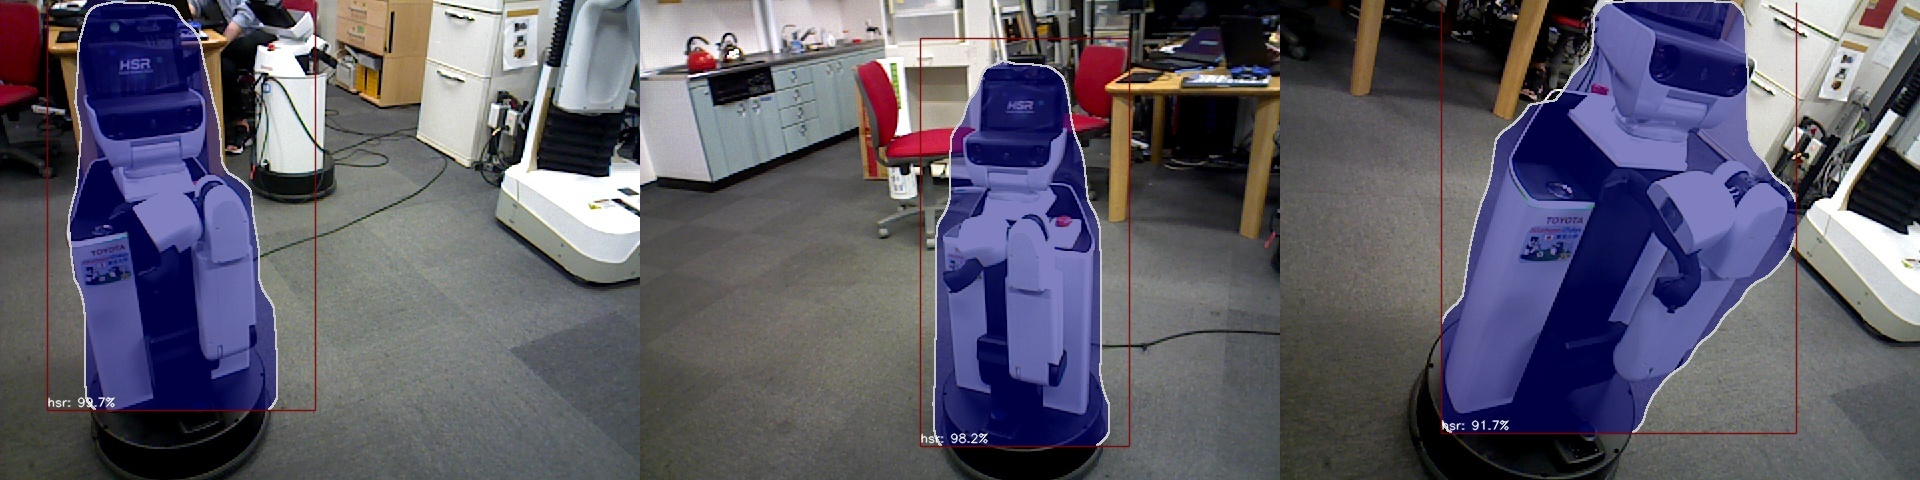
\includegraphics[width=0.8\columnwidth]{out.jpg}
   \caption{成功例}
  \label{figure:experiment}
 \end{center}
\end{figure}

\begin{figure}[htbp]
 \begin{center}
   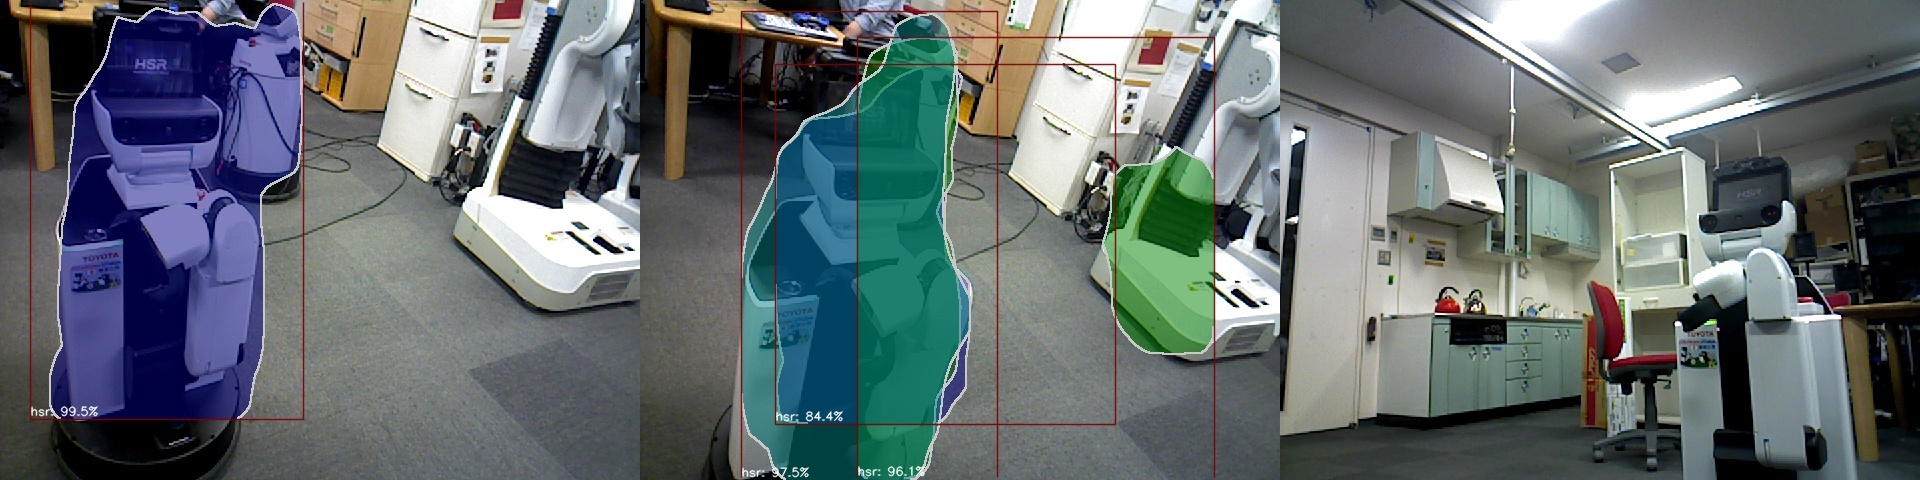
\includegraphics[width=0.8\columnwidth]{out_fail.jpg}
   \caption{失敗例}
  \label{figure:experiment_fail}
 \end{center}
\end{figure}

%% \section{はじめに}

%% 本稿はプログレスレポートのテンプレートである\cite{Sakai}.

%% 本稿における「、」や「。」は、\verb|make pub|を実行することで、「,」や「.」に変更される。

%% 図は\figref{nowprinting}や\tabref{sample}として参照する.

%% \begin{figure}[tbh]
%%  \begin{center}
%%   \begin{minipage}{0.3\columnwidth}
%%    \includegraphics[width=\columnwidth]{nowprinting.eps}
%%    \caption{eps図の参考例}
%%   \end{minipage}
%%   \hspace{0.15\columnwidth}
%%   \begin{minipage}{0.3\columnwidth}
%%    \includegraphics[width=\columnwidth]{dj.jpg}
%%    \caption{jpg図の参考例}
%%   \end{minipage}
%%   \label{figure:nowprinting}
%%  \end{center}
%% \end{figure}

%% \begin{table}[tbh]
%%  \begin{center}
%%   \begin{tabular}{|l|r|} \hline
%%   A1 & B1 \\
%%   A2 & B2 \\ \hline
%%   \end{tabular}
%%   \caption{図の参考例}
%%   \label{table:sample}
%%  \end{center}
%% \end{table}

%% \section{おわりに}

\bibliographystyle{junsrt}
\bibliography{p-report}

\end{document}

